% Licensed to the Apache Software Foundation (ASF) under one or more
% contributor license agreements. See the NOTICE file distributed with
% this work for additional information regarding copyright ownership.
% The ASF licenses this file to You under the Apache License, Version 2.0
% (the ``License''); you may not use this file except in compliance with
% the License. You may obtain a copy of the License at
%
% http://www.apache.org/licenses/LICENSE-2.0
%
% Unless required by applicable law or agreed to in writing, software
% distributed under the License is distributed on an ``AS IS'' BASIS,
% WITHOUT WARRANTIES OR CONDITIONS OF ANY KIND, either express or implied.
% See the License for the specific language governing permissions and
% limitations under the License.

\subsubsection{RSS Job Options}

You must fill in six more tabs to configure an RSS job.

\bigimage{RSS-edit-job-tab3}

\ifJDBCGuide
% Licensed to the Apache Software Foundation (ASF) under one or more
% contributor license agreements. See the NOTICE file distributed with
% this work for additional information regarding copyright ownership.
% The ASF licenses this file to You under the Apache License, Version 2.0
% (the ``License''); you may not use this file except in compliance with
% the License. You may obtain a copy of the License at
%
% http://www.apache.org/licenses/LICENSE-2.0
%
% Unless required by applicable law or agreed to in writing, software
% distributed under the License is distributed on an ``AS IS'' BASIS,
% WITHOUT WARRANTIES OR CONDITIONS OF ANY KIND, either express or implied.
% See the License for the specific language governing permissions and
% limitations under the License.

\begin{itemize}
\label{scheduling}

\item \textbf{Schedule type:} Whether you want to scan every document
once or dynamically recrawl content in your repository. 

When scanning every document once, the crawler marks all documents that
have been previously crawled in this job as potentially to be deleted,
adds all seed documents to its queue and marks them as pending, processes
pending documents, marking them completed as they are ingested, and then
deleted all of the documents that were not recrawled. A document might
not be recrawled because it no longer exists, or the job specification
might have been changed to no longer include the document.

When dynamically recrawling documents, the crawler does not start by
marking all documents as potentially deletable; instead, it begins with
all of the seed documents, and continues adding to its list, periodically
re-adding the initial seed documents. If a document is removed from the
source, it will expire in the expiration interval (see below).

\item \textbf{Expiration Interval (if continuous):} The length of the
interval (in minutes) that the appliance will retain a document
crawled by this job after the document no longer appears in the
repository. After this interval, the missing document will be removed
from the appliance's index and archive. Leave the expiration interval
blank to keep missing documents indexed in GTS.

\item \textbf{Recrawl interval:} If you are dynamically recrawling
documents, how long, in minutes, the crawler should wait before
crawling documents a second time.

\item \textbf{Reseed interval:} If you are dynamically recrawling
documents, how long, in minutes, the crawler should wait before
looking for new documents to crawl. \ifMeridioGuide This connector
identifies all documents for ingestion through seeding; if the reseed
interval is infinite, the job will not ingest documents placed in the
repository during run time. (The job automatically reseeds whenever it
is started.) The default interval of 60 minutes is an appropriate
reseed rate. \fi \ifFilenetGuide This connector identifies documents
for ingestion during seeding. If you change the document inclusion
criteria, reseeding is required to identify new documents. Similarly,
documents placed in the repository while the job is running will not
be identified until the crawl is reseeded.  (The job automatically
reseeds whenever it is started.) The default interval of 60 minutes is
an appropriate reseed rate. \fi

\item \textbf{Scheduled time:} Allows you to define a time you wish
the job to run using a series of selection boxes. The first box refers
to the day of the week you wish the job to run, with an option to have
the job run any day of the week. The second box allows you to select
the start hour, with an option to start the job at any hour. The third
box allows you to specify which minute after the hour that you wish
the job to start. The fourth box allows you to specify what months of
the year you wish the job to run, with an option for the job to run
any month. The last box allows you to specify the day of the month you
wish the job to start, including any day of month.


You can scroll through each of the five boxes in this setting using
the arrow keys on your keyboard or by using the scroll bar on the
right side of the box.  If you want to select more than one value,
hold down control as you scroll and click the values that you want to
select. This allows you to define multiple windows with the same
length, for example by selecting Monday, Wednesday, and Friday at the
same time.

\item \textbf{Maximum run time:} The longest you will allow the job to
run, in minutes. For example, if you want to start a job at 2 AM but
force it to stop at 8 AM so that users have access to the repository,
you should set this value to 360 minutes. If the job is not complete by the
end time, documents that have already been found will be indexed, and
the rest of the crawl will continue at the beginning of the next
schedule interval. 

When you have defined the scheduled time and assigned a maximum run
time, click on the ``Add Scheduled Time'' button. A new schedule box
will appear below the scheduled time, allowing you to create
additional scheduled run times.

Here is a sample schedule for a job that will run every
Monday from 2 am to 6 am:

\begin{changemargin}{-.3in}{0in} 
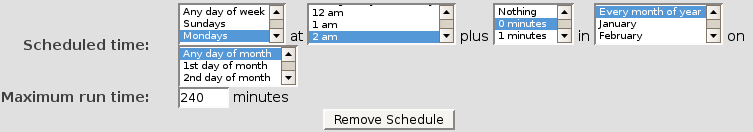
\includegraphics[width=300pt]{sample-schedule}
\end{changemargin}

If you do not have at least one scheduled time, the job will
only run when run manually (see page \pageref{ManageJobs}), and will
not automatically update the index on the appliance based on changes
to the repository.

You can remove a scheduled time by clicking the ``Remove Schedule''
button.

\end{itemize}

\fi

\ifCombinedConnectorGuide
This tab presents scheduling options. Here you can generate one or
more scheduled run times for the job. For a complete description of
the scheduling options, see the description starting on page
\pageref{scheduling}.
\fi

RSS feeds that are updated regularly will have documents fall off of the
end of the feed. If you are crawling continuously, those documents will
remain on the appliance until the expiration time set in this tab. If you
are crawling non-continuously, when the RSS connector job runs, documents
that are no longer in the feeds will be deleted from the appliance index.

\bigimage{RSS-edit-job-tab4}

On this tab, you are presented with a text box into which you should
enter the URLs of the feeds you wish this job to crawl. Each should be
on a separate line of the text box.

\bigimage{RSS-edit-job-tab5}

This tab allows you to apply some built-in canonicalization tools
to URLs before they are send to the MetaCarta ingestion system. If
canonicalization is not done properly, you risk either having duplicate
copies of the same document (for example, from having arguments to
a script in a different order but calling the script with the same
arguments) or having no copies of a document at all (for example, from
reordering the script arguments in a way that breaks the site being
crawled). The Connector Framework handles the reordering automatically,
but requires your intervention to decide which sites need to be reordered
and which do not. 

You can canonicalize based on regular expression; for more information on
regular expressions, please see the explanation in the next tab. Enter
a regular expression, a description of the URL (for your records only),
and then choose the types of canonicalization you would like enabled. You
have the following canonicalization options:

\begin{itemize}

\item \textbf{Reorder}: Take all arguments to any query in the URL and
order them programmatically. For example, a URL might include a query
string like ``article=foo0011\&format=fulltext.'' If the query string
were instead ``format=fulltext\&article=foo0011,'' the MetaCarta system
would treat it as a different document but it would contain the same
information. Normally, we recommend that you reorder all URLs, but
some sites require a specific order; for those sites, you should turn
reordering off.

\item \textbf{Remove JSP sessions}: Most of the time, you can safely
remove JSP session information from URLs. Uncheck this box if you find
that a particular site requires that you leave JSP session information
in the URL.

\item \textbf{Remove ASP sessions}: Most of the time, you can safely
remove ASP session information from URLs. Uncheck this box if you find
that a particular site requires that you leave ASP session information
in the URL.

\item \textbf{Remove PHP sessions}: Most of the time, you can safely
remove PHP session information from URLs. Uncheck this box if you find
that a particular site requires that you leave PHP session information
in the URL.

\item \textbf{Remove BV sessions}: Most of the time, you can safely
remove BV session information from URLs. Uncheck this box if you find
that a particular site requires that you leave BV session information
in the URL.

\end{itemize}

By default, all URLs are canonicalized in all five ways. 

\bigimage{RSS-edit-job-tab6}

This tab allows you to manipulate the URL ingested along with a
document. The URL ingested along with a document is by default the URL
from which the document was retrieved, but you may wish to provide a
different URL to be associated with the document. You can use regular
expressions to manipulate the URL. The example regular expression,
\verb+(.*)\:\/\/([A-Z|a-z|0-9|_|-|.]*)\/(.*)+, takes a URL, and breaks
it down into three parts; the protocol, the host server, and the file
path. The replacement string, \verb+1,''://www.example.com'',3+,
substitutes ``www.example.com'' for the host server.

You can specify more than one mapping. The mappings are applied in the
order in which they appear.

\note{If you are not familiar with regular expressions, there
are a variety of tutorials available on the web, including
\url{http://gnosis.cx/publish/}\linebreak\url{programming/regular_expressions.html}
and \url{http://perldoc.}\linebreak\url{perl.org/perlrequick.html}. If you still have
difficulty with these settings, please contact Customer Support (see
page \pageref{SupportContact}).}


\bigimage{RSS-edit-job-tab7}

\begin{itemize}

\item \textbf{Feed connect timeout (seconds):} A document fetch will time out after a period of inactivity. This field allows you to set the length of the timeout interval.

\item \textbf{Default feed refetch time (minutes)}: The feed may provide a suggested refetch interval. If no interval is provided, the crawler will use the interval you provide here.

\item \textbf{Minimum feed refetch time (minutes)}: If the suggested refetch interval is shorter than the interval specified here, the crawler will use this refresh interval.

\item \textbf{Bad feed refetch time (minutes)}: If the suggested refetch interval is shorter than the interval specified here, the crawler will use this refresh interval for bad feeds. 

\end{itemize}

\bigimage{RSS-edit-job-tab8}

\begin{itemize}

\item \textbf{Access Tokens:} If you wish to specify ACLs for files ingested through this job, you can specify them here. Simply enter one or more ACL identifiers into the field and click the ``Add'' button. The ACL identifiers will appear in a list. You can continue to add more ACL identifiers using the ``Add'' button, or remove them using the ``Delete'' button that appears next to each ACL identifier. By default, documents ingested through the RSS Connector will be accessible to all authorized search users. For assistance with this configuration, contact MetaCarta Support (see page \pageref{SupportContact}).

\end{itemize}

\bigimage{RSS-edit-job-tab9}

\begin{itemize}

\item \textbf{Metadata:} Here you can add additional metadata to be ingested along with documents crawled by this job. You should not overwrite existing metadata fields, such as collection name, using this tool.

\end{itemize}

\bigimage{RSS-edit-job-tab10}

Many commercial websites use ``chrome,'' or branding and advertising
information, that presents users with a number of browsing options
from the article they are reading. Unfortunately, this information
is often geographic, and can degrade the accuracy of the MetaCarta
indexing process. To solve this problem, the RSS site administrator
can include a ``dechromed'' version of the article, usually the article
itself without any additional information, in either the ``description''
or the ``content'' field of each article.

You can choose one of these three options:

\begin{itemize}

\item \textbf{No dechromed content:} There is no dechromed content in
this feed; the crawler should just fetch each document.

\item \textbf{Dechromed content, if present, in `description' field:}
The crawler will check the `description' field for content before fetching
the original document, and use anything it finds there preferentially.

\item \textbf{Dechromed content, if present, in `content' field:}
The crawler will check the `content' field for content before fetching
the original document, and use anything it finds there preferentially.

\end{itemize}

You can choose one of these two options:

\begin{itemize}

\item \textbf{Use chromed content if no dechromed content found:} If
there is no dechromed content, fetch the original document.

\item \textbf{Never use chromed content:} If there is no dechromed content,
do not index this document at all.

\end{itemize}

After entering this information, you will be taken to the status page
for this job:

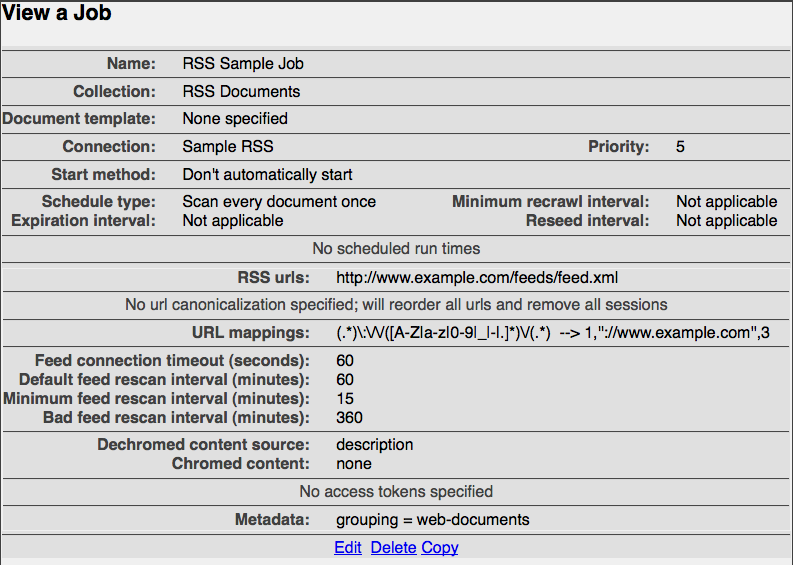
\includegraphics[width=300pt]{RSS-view-job-status}
